\begin{figure*}[t]
  \begin{center}
    \begin{tabular}{c}
      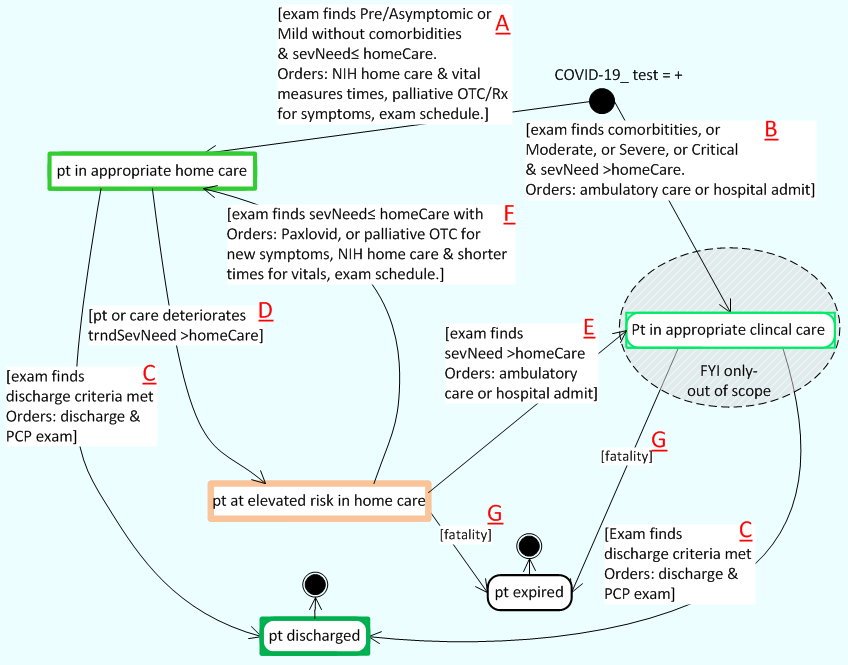
\includegraphics[scale=0.35]{cwp.png}
    \end{tabular}
  \end{center}
\caption{The CWP for remote COVID-19 patient care.}
\label{fig:cwp}
\end{figure*}

The purpose of \phware is remote monitoring that detects and analyzes seven vital signs to provide clinicians' with timely awareness of their outpatients' conditions and risk during home care, thereby supporting better decisions and enhancing patient safety. This purpose is, however, abstract and intangible. The CWP gives precise meaning to this purpose as a set of transformations on a complex object of work that is shared by activities in a distributed cognitive system.

To serve as an objective and operational definition of elevated risk due to home care, the work here adapts Medicare's 4-point severity-of-illness ratings \cite{Hornbrook2005OverviewOD,severity} and the CDC's Guidance on Home Care \cite{cdc}. The adaptation defines a \emph{Severity Level} less than two as mild, and a \emph{Home Care Capability Level} equal to two as typically appropriate. It then defines \emph{Elevated Outpatient Risk} from home care as either having a \emph{Trending Severity Level} or Severity Level greater than the Home Care Capability Level.

The CWP of actionable risk awareness was developed using these definitions as a finite state diagram, \figref{fig:cwp}, of the relevant care states patients can occupy, their associated risks, and the transition conditions among them. The transition conditions are based on the physician orders (\texttt{orders}), the current severity of the outpatient's condition assigned by a clinician's exam (\texttt{sevLvl}), the level of care at the outpatient's residence (\texttt{careCapLvl}), and the trending severity calculated from the remotely monitored longitudinal data as provided by
\phware\ cloud analytics (\texttt{trndSevLvl}). 

In the initial state (top) the patient has tested positive. The arc labeled \textbf{A} occurs when an exam shows symptoms of low severity and a provider orders home care with \phware. Outpatients remain in appropriate home care until either an exam finds discharge criteria met and ordered (\textbf{C}), or the trending severity level is greater than their care capability level (\textbf{D}). In such cases, patients are at an elevated risk in home care. They must not remain at an elevated risk in home care because there is a possible direct path to fatality (\textbf{G}). So a near future exam must either order admission (\textbf{E}), find their risk lower than what the analytics claimed, or make their risk lower with additional prescribed interventions (\textbf{F}). Patients who are admitted to hospital may eventually be discharged back to home care (\textbf{H}) or discharged directly (\textbf{C}). 

The declarative knowledge of the CWP specifies \emph{what} workflows solving the CWP must accomplish without depending on \emph{how} they do it. In this application, the CWP motivates the design, and then when the design is ready, the CWP is the property for formal verification that must be satisfied. 

The validation of the CWP for \phware\ is an interesting problem that is outside the scope of this paper but merits some discussion. Doctors reviewed the CWP using it as a kind of story-board whose rules at each arc are verified as appropriate care. One review noted that the CWP does not distinguish among causes of fatalities but concluded that any patient trending towards fatality must receive life-saving care regardless of co-morbidities, and so no change was required. The SPIN verification also served to validate the CWP and an example of that is given in \secref{sec:results}.

